%%%%%%%%%%%%%%%%%%%%%%%%%%%%%%%%%%%%%%%%%%
% Engineering problems / LaTeX Template
%		Semester 5
%		Institut d'Optique Graduate School
%%%%%%%%%%%%%%%%%%%%%%%%%%%%%%%%%%%%%%%%%%
%	5N-OptoElec-Sujet	
%%%%%%%%%%%%%%%%%%%%%%%%%%%%%%%%%%%%%%%%%%
%
% Created by:
%	Julien VILLEMEJANE - 05/may/2025
%	
%
%%%%%%%%%%%%%%%%%%%%%%%%%%%%%%%%%%%%%%%%%%
% Professional Newsletter Template
% LaTeX Template
% Version 1.0 (09/03/14)
%
% Created by:
% Bob Kerstetter (https://www.tug.org/texshowcase/) and extensively modified by:
% Vel (vel@latextemplates.com)
% 
% This template has been downloaded from:
% http://www.LaTeXTemplates.com
%
% License:
% CC BY-NC-SA 3.0 (http://creativecommons.org/li censes/by-nc-sa/3.0/)
%
%%%%%%%%%%%%%%%%%%%%%%%%%%%%%%%%%%%%%%%%%

\documentclass[a4paper,11pt,twoside]{book} % The default font size is 10pt; 11pt and 12pt are alternatives

%%%%%%%%%%%%%%%%%%%%%%%%%%%%%%%%%%%%%%%%%%%%%%%%%%%%%%%%%%%%%%%%%%%%%%%%%%%%%%%%%%%%%%%%%%%%%%%%%%%%%%%%%%%%%%%%%%%%%%%%%%%%%%%%%%%%%%%%%%%%%%%%%%%%%%%%%%%%%%%%%%%%%%%%%%%%%%%%%%%%%%%%%%%%%%%%%%%%%%%%%%%%%%%%%%%%%%%%%%%%%%%%%%%%%%%%%%%%%%%%%%%%%%%%%%%%
\usepackage{opto_elec_villemejane}

%%%%%%%%%%%%%%%%%%%%%%%%%%%%%%%%%%%%%%%%%%%%%%%%
%%%%%%%%%%%%%%%%%%%%%%%%%%%%%%%%%%%%%%%%%%%%%%%%
%%%%%%%%%%%%%%%%%%%%%%%%%%%%%%%%%%%%%%%%%%%%%%%%
%%%%%%%%%%%%%%%%%%%%%%%%%%%%%%%%%%%%%%%%%%%%%%%%
\begin{document}

\pagestyle{plain}

% Séances
\cleardoublepage
\ifodd\value{page}\else
  \hbox{}\newpage
\fi

\newpage
%\pagestyle{empty}

\begin{minipage}[c]{.25\linewidth}
	
\includegraphics[width=4cm]{images/LEnsE_IOGS.jpg}
\end{minipage} \hfill
\begin{minipage}[c]{.4\linewidth}

\begin{center}
\vspace{0.3cm}
{\Large \textsc{Opto-Électronique}}

\medskip

5N-027-SCI \qquad \textbf{\Large TD Asservissement}

\end{center}
\end{minipage}\hfill

%%%%%%%%%%%%%%%%%%%%%%%%%%%%%%%%%%
\section{TD Asservissement - Systèmes en boucle fermée}

Pour les exercices 1, 2 et 3, on considérera le schéma bloc suivant :

\begin{center}
{\Large
\begin{tikzpicture}
\sbEntree{E}
\sbComp{comp}{E}
\sbRelier[$G_E$]{E}{comp}

\sbStyleBloc{fill=schema_action}
\sbBloc{sys}{$A(j \omega)$}{comp}
\sbRelier[$\varepsilon$]{comp}{sys}

\sbStyleBlocDefaut
\sbSortie{S}{sys}
\sbRelier[$G_S$]{sys}{S}
\sbDecaleNoeudy[4]{S}{U} 
\sbStyleBloc{fill=schema_feed}
\sbBlocr{cap}{$B(j \omega)$}{U}
\sbStyleBlocDefaut
\sbRelieryx{sys-S}{cap}
\sbRelierxy[$G_M$]{cap}{comp}
\end{tikzpicture}
}
\end{center}


%%%%%%%%%%%%%%%%%%%%%%%%%%%%%%%%%%%%%%%%%%%%%%%%%%%%%%%
\subsection{Exercice 1 - Boucle ouverte et boucle fermée - Ordre 0}

Pour cet exercice, on considérera les fonctions de transfert suivantes : 

$A(j \omega) = K_A$ et $B(j \omega) = K_B$


\begin{enumerate}
	\item Donnez l'expression de $G_S$ en fonction de $G_E$, en \textbf{boucle ouverte}.
	\item Donnez l'expression de $G_M$ en fonction de $G_E$, en \textbf{boucle ouverte}.
		
	\item Donnez l'expression de la \textbf{fonction de transfert} $H(j \omega) = G_S / G_E$, en \textbf{boucle fermée}.
	\item Calculez la \textbf{fonction de transfert} pour les valeurs suivantes de $K_A$ et $K_B$ :
	\begin{itemize}
		\item $K_A = 1$ et $K_B = 1$
		\item $K_A = 10$ et $K_B = 1$
		\item $K_A = 100$ et $K_B = 1$
		\item $K_A = 1$ et $K_B = 10^{-2}$
		\item $K_A = 10^7$ et $K_B = 10^{-4}$ (cas amplificateur inverseur par exemple)
	\end{itemize}
	\item Quelles sont les limites de $H$ lorsque $K_A K_B >> 1$ ? Lorsque $K_A K_B << 1$ ?
\end{enumerate}

%%%%%%%%%%%%%%%%%%%%%%%%%%%%%%%%%%%%%%%%%%%%%%%%%%%%%%%
\subsection{Exercice 2 - Boucle ouverte et boucle fermée - Ordre 1}

Pour cet exercice, on considérera les fonctions de transfert suivantes : 

$A(j \omega) = \frac{K_A}{1 + T_A j \omega}$ et $B(j \omega) = K_B$

\begin{enumerate}
	\item Donnez l'expression de la \textbf{fonction de transfert} $H(j \omega) = G_S / G_E$, en \textbf{boucle fermée}. 
	\item Mettez cette expression sous \textbf{forme canonique} et donnez les \textbf{principales caractéristiques} du système obtenu.
	\item Calculez ces valeurs caractéristiques pour les valeurs suivantes de $K_A$, $K_B$ et $T_A$ :
	\begin{itemize}
		\item $K_A = 1$, $K_B = 1$ et $T_A = 100\operatorname{ms}$
		\item $K_A = 10$, $K_B = 1$ et $T_A = 100\operatorname{ms}$
		\item $K_A = 10^7$, $K_B = 10^{-4}$ et $T_A = 100\operatorname{ms}$ (cas amplificateur inverseur par exemple)
	\end{itemize}
\end{enumerate}


\newpage
%%%%%%%%%%%%%%%%%%%%%%%%%%%%%%%%%%%%%%%%%%%%%%%%%%%%%%%
\subsection{Exercice 3 - Boucle ouverte et boucle fermée - Ordre 1}

Pour cet exercice, on considérera les fonctions de transfert suivantes : 

$A(j \omega) = K_A$ et $B(j \omega) = \frac{K_B}{1 + T_B j \omega}$

On donne l'expression suivante pour $H(j \omega) = G_S / G_E$ :

$$H(j \omega) = \frac{K_A}{1 + K_A K_B} \cdot \frac{1 + T_B j \omega}{1 + \frac{T_B}{1 + K_A K_B} j \omega}$$


\begin{enumerate}
	\item Tracez le gain de cette fonction de transfert dans les deux conditions suivantes :
	\begin{itemize}
		\item $K_A K_B > 1$
		\item $K_A K_B < 1$		
	\end{itemize}
	\item Donnez également l'expression du gain statique de ce système dans les deux conditions précédentes.
	\item Donnez également l'expression du rapport de la constante de temps du système bouclé sur celle du système A dans les deux conditions précédentes.
\end{enumerate}


\noindent\hrulefill

%%%%%%%%%%%%%%%%%%%%%%
%%%%%%%%%%%%%%%%%%%%%%
Pour les exercices 4 et 5, on considérera le schéma bloc suivant :


\begin{center}
{\Large
\begin{tikzpicture}
\sbEntree{E}
\sbComp{comp}{E}
\sbRelier[$G_E$]{E}{comp}
\sbStyleBloc{fill=schema_PID}
\sbBloc{reg}{$C(j \omega)$}{comp}
\sbRelier[$\varepsilon$]{comp}{reg}
\sbStyleBloc{fill=schema_action}
\sbBloc{sys}{$A(j \omega)$}{reg}
\sbStyleBlocDefaut
\sbRelier[$G_u$]{reg}{sys}
\sbSortie{S}{sys}
\sbRelier[$G_S$]{sys}{S}
\sbDecaleNoeudy[4]{S}{U}
\sbStyleBloc{fill=schema_feed}
\sbBlocr{cap}{$B(j \omega)$}{U}
\sbStyleBlocDefaut
\sbRelieryx{sys-S}{cap}
\sbRelierxy[$G_M$]{cap}{comp}
\end{tikzpicture}
}
\end{center}


%%%%%%%%%%%%%%%%%%%%%%%%%%%%%%%%%%%%%%%%%%%%%%%%%%%%%%%
\subsection{Exercice 4 - Correcteur P}

Pour cet exercice, on considérera les fonctions de transfert suivantes : 

$A(j \omega) = \frac{K_A}{1 + T_A j \omega}$, $B(j \omega) = K_B$ et $C(j \omega) = K_C$ 

\begin{enumerate}
	\item Donnez l'expression de $G_M$ en fonction de $G_E$, en \textbf{boucle ouverte}.
		
	\item Donnez l'expression de la \textbf{fonction de transfert} $H(j \omega) = G_S / G_E$, en \textbf{boucle fermée}.
	\item Mettez cette expression sous \textbf{forme canonique} et donnez les \textbf{principales caractéristiques} du système obtenu.
	\item Calculez ces valeurs caractéristiques pour les valeurs suivantes de $K_A$, $K_B$ et $T_A$ :
	\begin{itemize}
		\item $K_A = 1$, $K_B = 1$, $K_C = 10$ et $T_A = 100\operatorname{ms}$
		\item $K_A = 1$, $K_B = 10^{-2}$, $K_C = 10$ et $T_A = 100\operatorname{ms}$
	\end{itemize}
\end{enumerate}



%%%%%%%%%%%%%%%%%%%%%%%%%%%%%%%%%%%%%%%%%%%%%%%%%%%%%%%
\subsection{Exercice 5 - Correcteur PI}

Pour cet exercice, on considérera les fonctions de transfert suivantes : 

$A(j \omega) = \frac{K_A}{1 + T_A j \omega}$, $B(j \omega) = K_B$ et $C(j \omega) = K_C + \frac{1}{T_I j \omega}$ 

\bigskip

\begin{enumerate}
	\item Comparez les diagrammes de Bode en gain et les réponses indicielles suivants.
	\item Concluez sur le rôle des correcteurs proportionnel et intégral.
\end{enumerate}

\begin{center}
	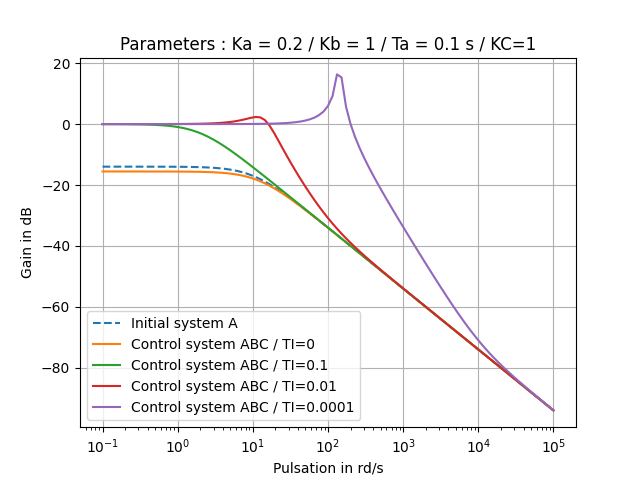
\includegraphics[width=0.8\textwidth]{images/A_0_B_0_CI_1_bode_comp1.png}
	
	Comparaison du diagramme de Bode en gain en fonction de la constante de temps de l'intégrateur - $K_C = 1$.
\end{center}

\begin{center}
	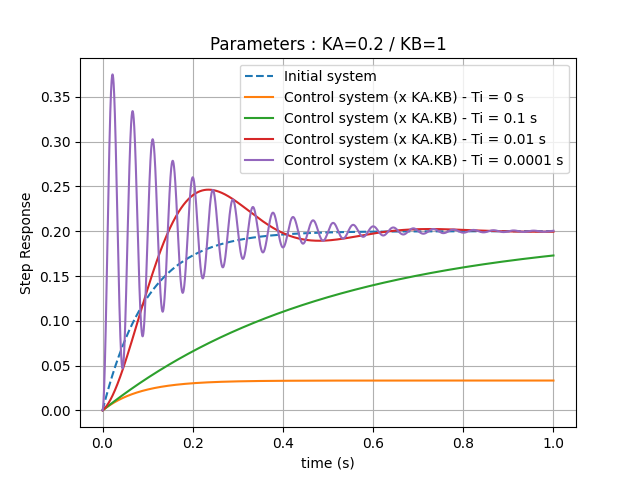
\includegraphics[width=0.8\textwidth]{images/A_0_B_0_CI_1_step_comp1.png}
	
	Comparaison de la réponses indicielle en fonction de la constante de temps de l'intégrateur - $K_C = 1$.
\end{center}


\begin{center}
	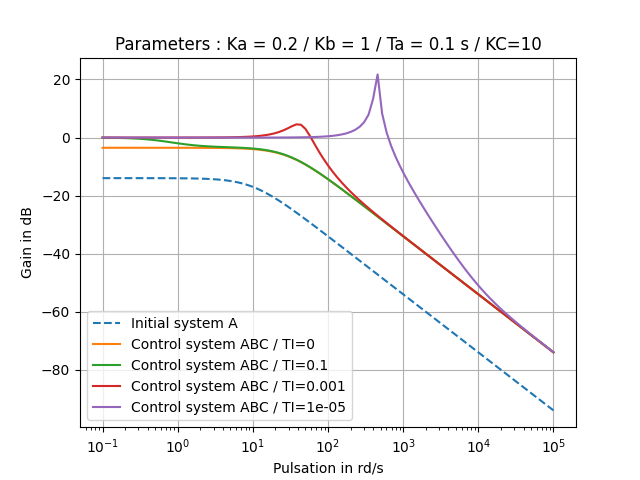
\includegraphics[width=0.8\textwidth]{images/A_0_B_0_CI_1_bode_comp2.png}
	
	Comparaison du diagramme de Bode en gain en fonction de la constante de temps de l'intégrateur - $K_C = 10$.
\end{center}

\begin{center}
	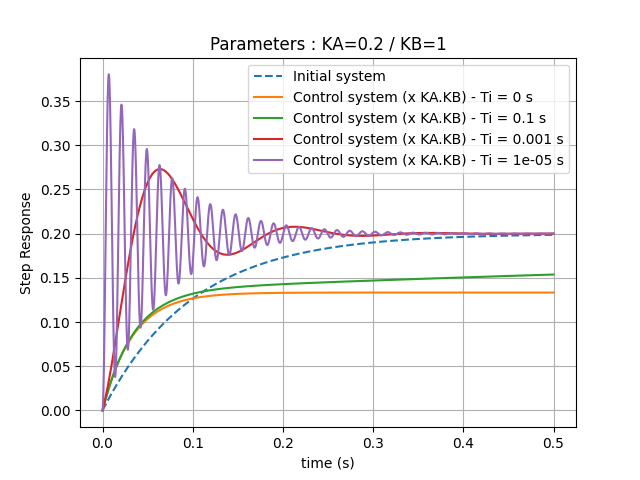
\includegraphics[width=0.8\textwidth]{images/A_0_B_0_CI_1_step_comp2.png}
	
	 Comparaison de la réponses indicielle en fonction de la constante de temps de l'intégrateur - $K_C = 10$.
\end{center}



%%%%%%%%%%%%%%%%%%%%%%%%%%%%%%%%%%%%%%%%%%%%%%%%%%%%%%%


\end{document}


